\documentclass{standalone}
\usepackage{tikz}
\usetikzlibrary{patterns, positioning}

\begin{document}
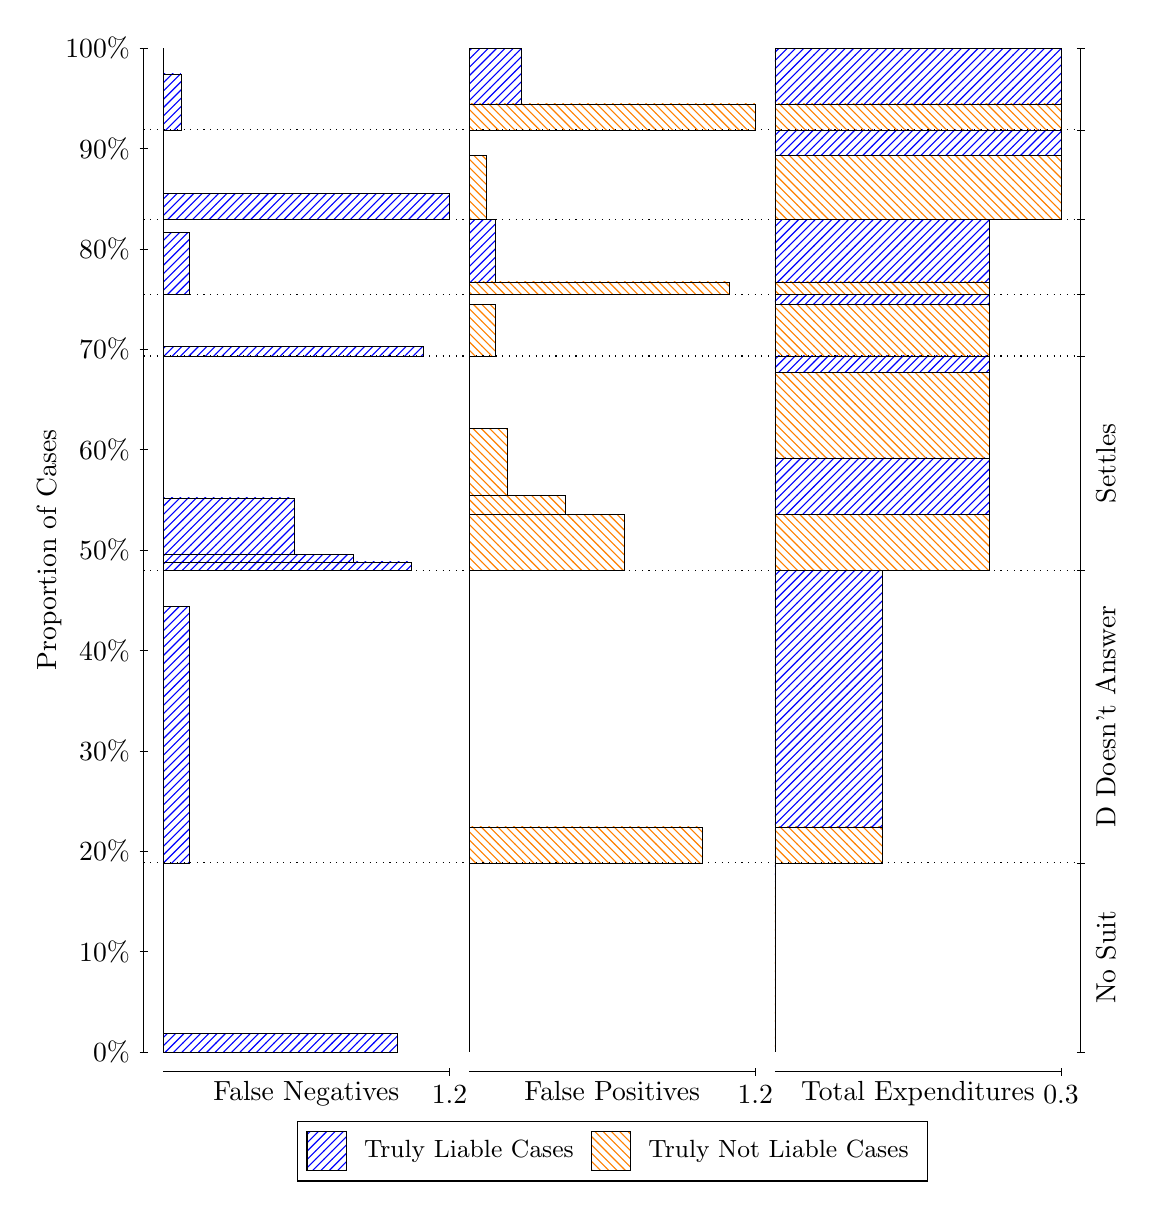
\begin{tikzpicture}
\draw[black, very thin] (1.5,1.75) -- (1.5,14.5);
\node[rotate=90, anchor=center] at (0.3, 8.125) {Proportion of Cases};
\draw[black, very thin] (1.45,1.75) -- (1.55,1.75);
\node[anchor=east] at (1.45, 1.75) {0\%};
\draw[black, very thin] (1.45,3.025) -- (1.55,3.025);
\node[anchor=east] at (1.45, 3.025) {10\%};
\draw[black, very thin] (1.45,4.3) -- (1.55,4.3);
\node[anchor=east] at (1.45, 4.3) {20\%};
\draw[black, very thin] (1.45,5.575) -- (1.55,5.575);
\node[anchor=east] at (1.45, 5.575) {30\%};
\draw[black, very thin] (1.45,6.85) -- (1.55,6.85);
\node[anchor=east] at (1.45, 6.85) {40\%};
\draw[black, very thin] (1.45,8.125) -- (1.55,8.125);
\node[anchor=east] at (1.45, 8.125) {50\%};
\draw[black, very thin] (1.45,9.4) -- (1.55,9.4);
\node[anchor=east] at (1.45, 9.4) {60\%};
\draw[black, very thin] (1.45,10.675) -- (1.55,10.675);
\node[anchor=east] at (1.45, 10.675) {70\%};
\draw[black, very thin] (1.45,11.95) -- (1.55,11.95);
\node[anchor=east] at (1.45, 11.95) {80\%};
\draw[black, very thin] (1.45,13.225) -- (1.55,13.225);
\node[anchor=east] at (1.45, 13.225) {90\%};
\draw[black, very thin] (1.45,14.5) -- (1.55,14.5);
\node[anchor=east] at (1.45, 14.5) {100\%};

\draw[black, very thin] (13.4,1.75) -- (13.4,14.5);
\draw[black, very thin] (13.35,1.75) -- (13.45,1.75);
\node[anchor=west] at (13.35, 1.75) {};
\draw[black, very thin] (13.35,4.1507) -- (13.45,4.1507);
\node[anchor=west] at (13.35, 4.1507) {};
\draw[black, very thin] (13.35,7.8663) -- (13.45,7.8663);
\node[anchor=west] at (13.35, 7.8663) {};
\draw[black, very thin] (13.35,10.589) -- (13.45,10.589);
\node[anchor=west] at (13.35, 10.589) {};
\draw[black, very thin] (13.35,11.369) -- (13.45,11.369);
\node[anchor=west] at (13.35, 11.369) {};
\draw[black, very thin] (13.35,12.323) -- (13.45,12.323);
\node[anchor=west] at (13.35, 12.323) {};
\draw[black, very thin] (13.35,13.461) -- (13.45,13.461);
\node[anchor=west] at (13.35, 13.461) {};
\draw[black, very thin] (13.35,14.5) -- (13.45,14.5);
\node[anchor=west] at (13.35, 14.5) {};

\draw[black, very thin, pattern color=blue, pattern=north east lines] (1.75,1.75) rectangle (4.716,1.991);
\draw[black, very thin, pattern color=orange, pattern=north west lines] (1.75,1.991) rectangle (1.75,4.1507);
\draw[black, very thin, pattern color=blue, pattern=north east lines] (1.75,4.1507) rectangle (2.0837,7.4086);
\draw[black, very thin, pattern color=orange, pattern=north west lines] (1.75,7.4086) rectangle (1.75,7.8663);
\draw[black, very thin, pattern color=blue, pattern=north east lines] (1.75,7.8663) rectangle (4.9014,7.9746);
\draw[black, very thin, pattern color=blue, pattern=north east lines] (1.75,7.9746) rectangle (4.1599,8.0725);
\draw[black, very thin, pattern color=blue, pattern=north east lines] (1.75,8.0725) rectangle (3.4184,8.788);
\draw[black, very thin, pattern color=orange, pattern=north west lines] (1.75,8.788) rectangle (1.75,10.589);
\draw[black, very thin, pattern color=blue, pattern=north east lines] (1.75,10.589) rectangle (5.0497,10.713);
\draw[black, very thin, pattern color=orange, pattern=north west lines] (1.75,10.713) rectangle (1.75,11.369);
\draw[black, very thin, pattern color=blue, pattern=north east lines] (1.75,11.369) rectangle (2.0837,12.161);
\draw[black, very thin, pattern color=orange, pattern=north west lines] (1.75,12.161) rectangle (1.75,12.323);
\draw[black, very thin, pattern color=blue, pattern=north east lines] (1.75,12.323) rectangle (5.3833,12.652);
\draw[black, very thin, pattern color=orange, pattern=north west lines] (1.75,12.652) rectangle (1.75,13.461);
\draw[black, very thin, pattern color=blue, pattern=north east lines] (1.75,13.461) rectangle (1.9724,14.171);
\draw[black, very thin, pattern color=orange, pattern=north west lines] (1.75,14.171) rectangle (1.75,14.5);
\draw[black, very thin, pattern color=orange, pattern=north west lines] (5.6333,1.75) rectangle (5.6333,3.9097);
\draw[black, very thin, pattern color=blue, pattern=north east lines] (5.6333,3.9097) rectangle (5.6333,4.1507);
\draw[black, very thin, pattern color=orange, pattern=north west lines] (5.6333,4.1507) rectangle (8.5993,4.6084);
\draw[black, very thin, pattern color=blue, pattern=north east lines] (5.6333,4.6084) rectangle (5.6333,7.8663);
\draw[black, very thin, pattern color=orange, pattern=north west lines] (5.6333,7.8663) rectangle (7.5983,8.5791);
\draw[black, very thin, pattern color=orange, pattern=north west lines] (5.6333,8.5791) rectangle (6.8568,8.8183);
\draw[black, very thin, pattern color=orange, pattern=north west lines] (5.6333,8.8183) rectangle (6.1153,9.6671);
\draw[black, very thin, pattern color=blue, pattern=north east lines] (5.6333,9.6671) rectangle (5.6333,10.589);
\draw[black, very thin, pattern color=orange, pattern=north west lines] (5.6333,10.589) rectangle (5.967,11.245);
\draw[black, very thin, pattern color=blue, pattern=north east lines] (5.6333,11.245) rectangle (5.6333,11.369);
\draw[black, very thin, pattern color=orange, pattern=north west lines] (5.6333,11.369) rectangle (8.933,11.531);
\draw[black, very thin, pattern color=blue, pattern=north east lines] (5.6333,11.531) rectangle (5.967,12.323);
\draw[black, very thin, pattern color=orange, pattern=north west lines] (5.6333,12.323) rectangle (5.8558,13.132);
\draw[black, very thin, pattern color=blue, pattern=north east lines] (5.6333,13.132) rectangle (5.6333,13.461);
\draw[black, very thin, pattern color=orange, pattern=north west lines] (5.6333,13.461) rectangle (9.2667,13.791);
\draw[black, very thin, pattern color=blue, pattern=north east lines] (5.6333,13.791) rectangle (6.3007,14.5);
\draw[black, very thin, pattern color=orange, pattern=north west lines] (9.5167,1.75) rectangle (9.5167,3.9097);
\draw[black, very thin, pattern color=blue, pattern=north east lines] (9.5167,3.9097) rectangle (9.5167,4.1507);
\draw[black, very thin, pattern color=orange, pattern=north west lines] (9.5167,4.1507) rectangle (10.879,4.6084);
\draw[black, very thin, pattern color=blue, pattern=north east lines] (9.5167,4.6084) rectangle (10.879,7.8663);
\draw[black, very thin, pattern color=orange, pattern=north west lines] (9.5167,7.8663) rectangle (12.242,8.5791);
\draw[black, very thin, pattern color=blue, pattern=north east lines] (9.5167,8.5791) rectangle (12.242,9.2947);
\draw[black, very thin, pattern color=orange, pattern=north west lines] (9.5167,9.2947) rectangle (12.242,10.383);
\draw[black, very thin, pattern color=blue, pattern=north east lines] (9.5167,10.383) rectangle (12.242,10.589);
\draw[black, very thin, pattern color=orange, pattern=north west lines] (9.5167,10.589) rectangle (12.242,11.245);
\draw[black, very thin, pattern color=blue, pattern=north east lines] (9.5167,11.245) rectangle (12.242,11.369);
\draw[black, very thin, pattern color=orange, pattern=north west lines] (9.5167,11.369) rectangle (12.242,11.531);
\draw[black, very thin, pattern color=blue, pattern=north east lines] (9.5167,11.531) rectangle (12.242,12.323);
\draw[black, very thin, pattern color=orange, pattern=north west lines] (9.5167,12.323) rectangle (13.15,13.132);
\draw[black, very thin, pattern color=blue, pattern=north east lines] (9.5167,13.132) rectangle (13.15,13.461);
\draw[black, very thin, pattern color=orange, pattern=north west lines] (9.5167,13.461) rectangle (13.15,13.791);
\draw[black, very thin, pattern color=blue, pattern=north east lines] (9.5167,13.791) rectangle (13.15,14.5);
\draw[black, dotted] (1.5,4.1507) -- (13.4,4.1507);
\draw[black, dotted] (1.5,7.8663) -- (13.4,7.8663);
\draw[black, dotted] (1.5,10.589) -- (13.4,10.589);
\draw[black, dotted] (1.5,11.369) -- (13.4,11.369);
\draw[black, dotted] (1.5,12.323) -- (13.4,12.323);
\draw[black, dotted] (1.5,13.461) -- (13.4,13.461);
\draw[black, very thin] (1.75,1.5) -- (5.3833,1.5);
\node[anchor=north] at (3.5667, 1.5) {False Negatives};
\draw[black, very thin] (5.3833,1.45) -- (5.3833,1.55);
\node[anchor=north] at (5.3833, 1.45) {1.2};

\draw[black, very thin] (5.6333,1.5) -- (9.2667,1.5);
\node[anchor=north] at (7.45, 1.5) {False Positives};
\draw[black, very thin] (9.2667,1.45) -- (9.2667,1.55);
\node[anchor=north] at (9.2667, 1.45) {1.2};

\draw[black, very thin] (9.5167,1.5) -- (13.15,1.5);
\node[anchor=north] at (11.333, 1.5) {Total Expenditures};
\draw[black, very thin] (13.15,1.45) -- (13.15,1.55);
\node[anchor=north] at (13.15, 1.45) {0.3};

\node[black, centered, rotate=90] at (13.72, 2.9503) {No Suit};
\node[black, centered, rotate=90] at (13.72, 6.0085) {D Doesn't Answer};
\node[black, centered, rotate=90] at (13.72, 9.2276) {Settles};





\draw (7.449999999999999,1.5) node[draw=none] (baseCoordinate) {};
\begin{scope}[align=center]
        \matrix[scale=0.5, draw=black, below=0.5cm of baseCoordinate, nodes={draw}, column sep=0.1cm]{
            \node[rectangle, draw, minimum width=0.5cm, minimum height=0.5cm, pattern=north east lines, pattern color=blue] {}; &
            \node[draw=none, font=\small] (B) {Truly Liable Cases}; &
            \node[rectangle, draw, minimum width=0.5cm, minimum height=0.5cm, pattern=north west lines, pattern color=orange] {}; &
            \node[draw=none, font=\small] (B) {Truly Not Liable Cases}; \\
            };
\end{scope}

\end{tikzpicture}
\end{document}